%
% $RCSfile: lifecycle.tex,v $
%
% Copyright (c) 2001-2004. Christian Heller. All rights reserved.
%
% Permission is granted to copy, distribute and/or modify this document
% under the terms of the GNU Free Documentation License, Version 1.1
% or any later version published by the Free Software Foundation;
% with no Invariant Sections, with no Front-Cover Texts and with no Back-Cover
% Texts. A copy of the license is included in the section entitled
% "GNU Free Documentation License".
%
% http://www.cybop.net
% - Cybernetics Oriented Programming -
%
% http://www.resmedicinae.org
% - Information in Medicine -
%
% @author Christian Heller <christian.heller@tuxtax.de>
% @author Jens Bohl <info@jens-bohl.de>
%

\section{An Extended Component Lifecycle}
\label{an_extended_component_lifecycle_heading}

The CYBOP lifecycle of components is an extension of the lifecycle idea of
Apache -- basically the same idea but another background and realization.\\
All \emph{Whole-Part associations} between objects were organized under the
rules of the component lifecycle. The relations were created and destroyed in
a sequence of lifecycle steps. These steps are realized as method calls on the
components (figure \ref{component_lifecycle_figure}).

\begin{figure}[ht]
    \begin{center}
       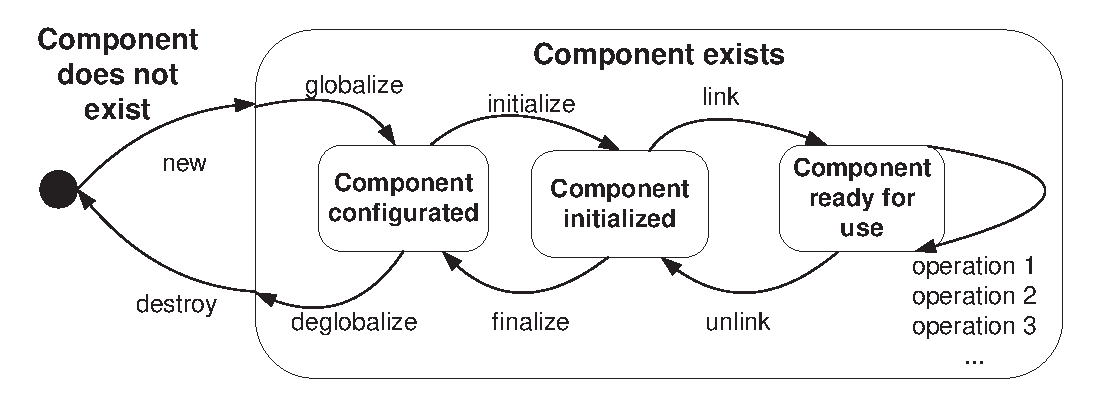
\includegraphics[scale=0.4]{eps/lebenszyklusEng.eps}
       \caption{State Diagram of CYBOB's Component Lifecycle}
       \label{component_lifecycle_figure}
    \end{center}
\end{figure}

Contrary to Apache's lifecycle, this one introduces a \emph{globalize} method
by which global parameters can be forwarded throughout the whole framework.
Static methods or \emph{manager} classes such become superfluous.
Analogous to the lifecycle of organic cells where the genetic information in form
of a Desoxyribo Nuklein Acid (DNA) is shared before separation, the globalize
method allows to forward a configuration object to any new instance.

